% Ubah judul dan label berikut sesuai dengan yang diinginkan.
\section{Related Works}
\label{sec:tinjauanpustaka}

% Ubah bagian-bagian berikut dengan isi dari tinjauan pustaka
\subsection{Previous Research}
Polynomial Regression Method is an approximation method for data that has been provided before. The output of the Polynomial Regression method is a mathematical formula based on the data that has been provided. Polynomial regression can work efficiently even with a non-linear model
\citet{ref_regresi}. There is a basic formula of Polynomial Regression: 
\begin{equation}
  y = a_0 + a_1x + a_2x^2 + \ldots + a_nx^n
\end{equation} 
where $y$ is the dependent variable, $x$ is the independent variable, $a_0$ is the intercept, $a_1$ is the coefficient of $x$, $a_2$ is the coefficient of $x^2$, and so on until $a_n$ is the coefficient of $x^n$. 

The Previous Research of Omnivision Camera calibration is using Polynomial Regression to calibrate Omnivision Camera. The $y$ is the distance from the camera to the object in real world, $x$ is distance of object from center of camera. The result of the Polynomial Regression is a mathematical formula that can be used to calculate the distance from the camera to the object.

The next step of using a Polinomial Regression is to change polar coordinates into cartesian coordinates. So the final output of the camera callibration is the cartesian coordinates of the object in the real world. And the input is cartesian coordinates of the object in the image. Here is the algorithm to calculate the cartesian coordinates of the object in the real world: 
\begin{algorithm}
  \caption{Data Calculation using Polynomial Regression}\label{alg:calculate_coordinates}
  \begin{algorithmic}[1]
  \Procedure{CalculateCoordinatesAndAngles}{}
      \State \text{Compute } $dx \gets x - x\_center\_cam$
      \State \text{Compute } $dy \gets y\_center\_cam - y$
      \State \text{Compute } $\theta \gets \arctan(\frac{dy}{dx})$
      \State \text{Compute } $x\_world \gets jarak\_sebenarnya \times \cos(\theta)$
      \State \text{Compute } $y\_world \gets jarak\_sebenarnya \times \sin(\theta)$
  \EndProcedure
  \end{algorithmic}
\end{algorithm}

With $x\_world$ representing the x coordinate in the field and $y\_world$ representing the y coordinate in the field. Then the position of the object in the field can be obtained.

\subsection{Basic Theory/Concept}

\subsubsection{Callibration}
\label{sec:callibration}

Callibration is a process to rearrange the parameters in a system to match the standards that have been determined before. Callibration is widely used in measurement systems, robotic systems, automation systems, and other systems. Callibration on the camera is a process to rearrange the camera so that it can see objects at a distance that matches the actual distance. Camera callibration is usually done by software by entering camera data into the computation process. The process can change camera data according to the actual data.

\subsubsection{Omnivision Camera}
\label{sec:omnivision}
\begin{figure}[ht]
    \centering
    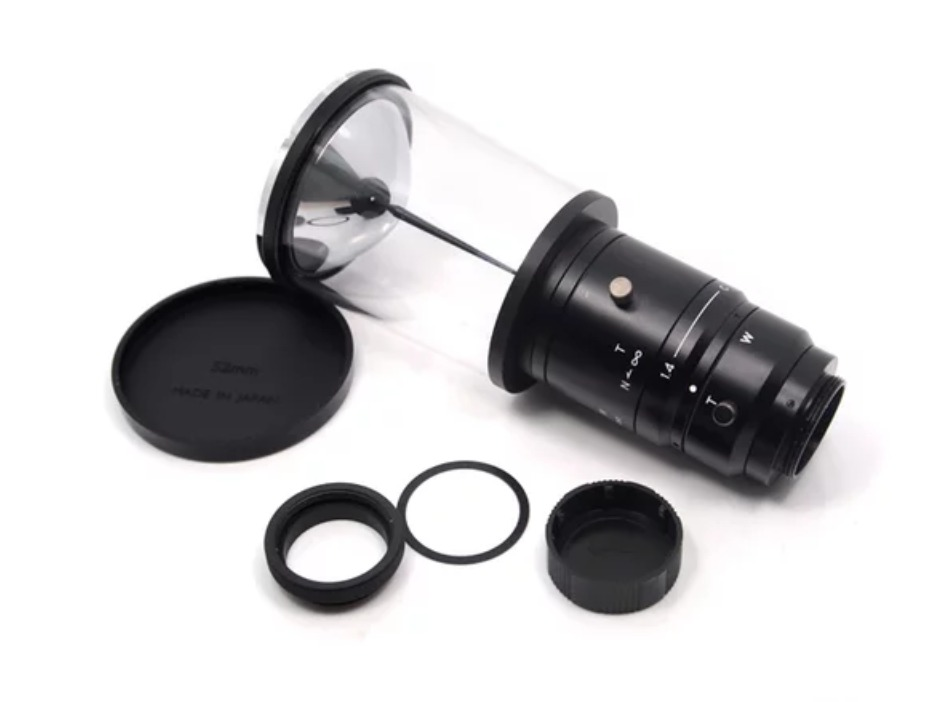
\includegraphics[width=6cm]{gambar/omnivisino2.jpeg}
    \caption{Omnivision Camera.}
    \label{fig:omnivision}
\end{figure}

Omnivision Camera is a camera that can see 360 degrees around the camera \citet{ref_kamera_omni}. The range of view of the Omnivision Camera is unlimited depending on the resolution of the camera itself and the construction of the mirror. Basically, the Omnivision Camera is a regular camera that is shot into a convex mirror so that the camera's view can be in all directions.

\begin{figure}[ht]
  \centering
  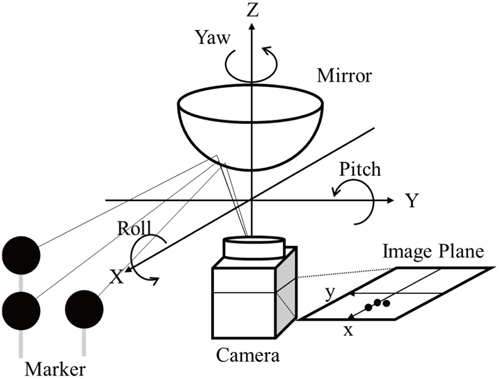
\includegraphics[width=6cm]{gambar/omnivision3.jpg}
  \caption{Basic Concept of Omnivision Camera.}
  \label{fig:omnivision3}
\end{figure}

From the figure above, the Omnivision camera is a camera that faces 90 degrees to the flat plane and is shot into a convex mirror. The convex mirror will reflect the light that enters the camera and vice versa. This work makes the Omnivision camera can see in all directions.

\subsubsection{Neural Network}
\label{sec:nn}
% \begin{figure}[ht]
%     \centering
  
%     % Ubah dengan nama file gambar dan ukuran yang akan digunakan
%     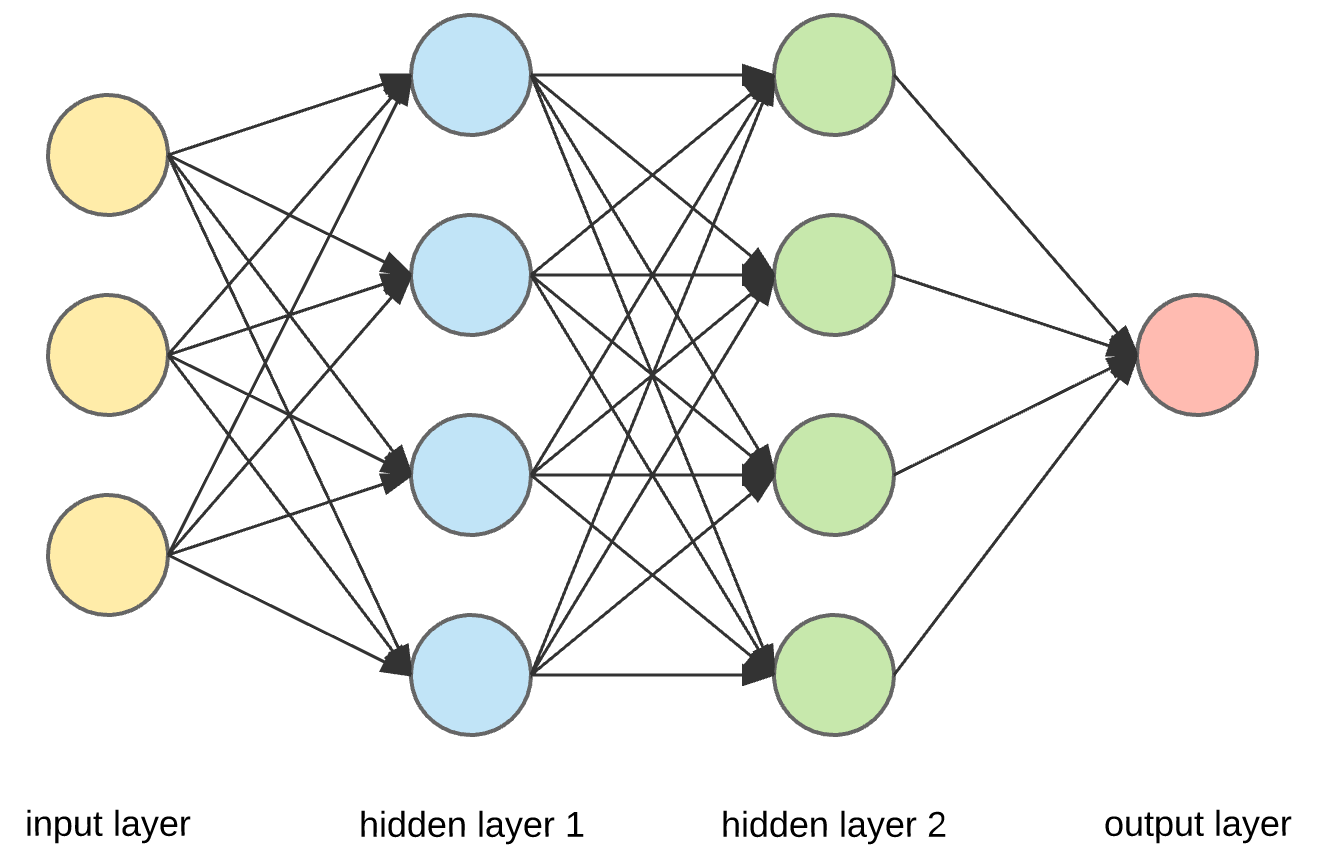
\includegraphics[width=8cm]{gambar/nn.png}
  
%     % Ubah dengan keterangan gambar yang diinginkan
%     \caption{Neural Network.}
%     \label{fig:nn}
% \end{figure}

Neural Network is a part of Machine Learning. Neural Network is created to overcome nonlinearity problems in a model \citet{ref_neural_network}. Basically, Neural Network is just a collection of Neurons connected by a Weight and Bias. In addition to Weight and Bias, there is also a forward propagation using an activation function or commonly called a transfer function. In addition to forward propagation, there is also backward propagation using a loss function.

\subsubsection{\emph{Activation Function}}
\label{sec:activation_function}

Activation function is a function used to transfer data at each layer in the Neural Network. In the Neural Network, the Activation function acts as forward propagation, which is the journey from the input layer to the output layer. Some activation functions have saturation values usually valued at 1, for example, Sigmoid which is valued in the range 0 to 1. There is also another activation function, namely tanh which is valued in the range -1 to 1 \citet{ref_activation_function}.

\subsubsection{\emph{Loss Function}}
\label{sec:loss_function}

Loss function is part of the Neural Network that aims to provide feedback to the model about the good or bad phase of training. Loss function in the Neural Network works on the Backward Propagation path, which is from the output layer to the input layer. There are several types of loss functions, one of which is MSE (Mean Squared Error). MSE loss function is better used on data with low fluctuation values \citet{ref_loss_function}.

Not only the loss function, there is another theory called Optimizer. Optimizer is an algorithm that can be used to determine the learning rate of the training system. The learning rate in the Neural Network is used to set how fast the model will converge to its data.

\subsubsection{\emph{Mobile Robot}}
\label{sec:mobile_robot}
\begin{figure}[ht]
    \centering
  
    % Ubah dengan nama file gambar dan ukuran yang akan digunakan
    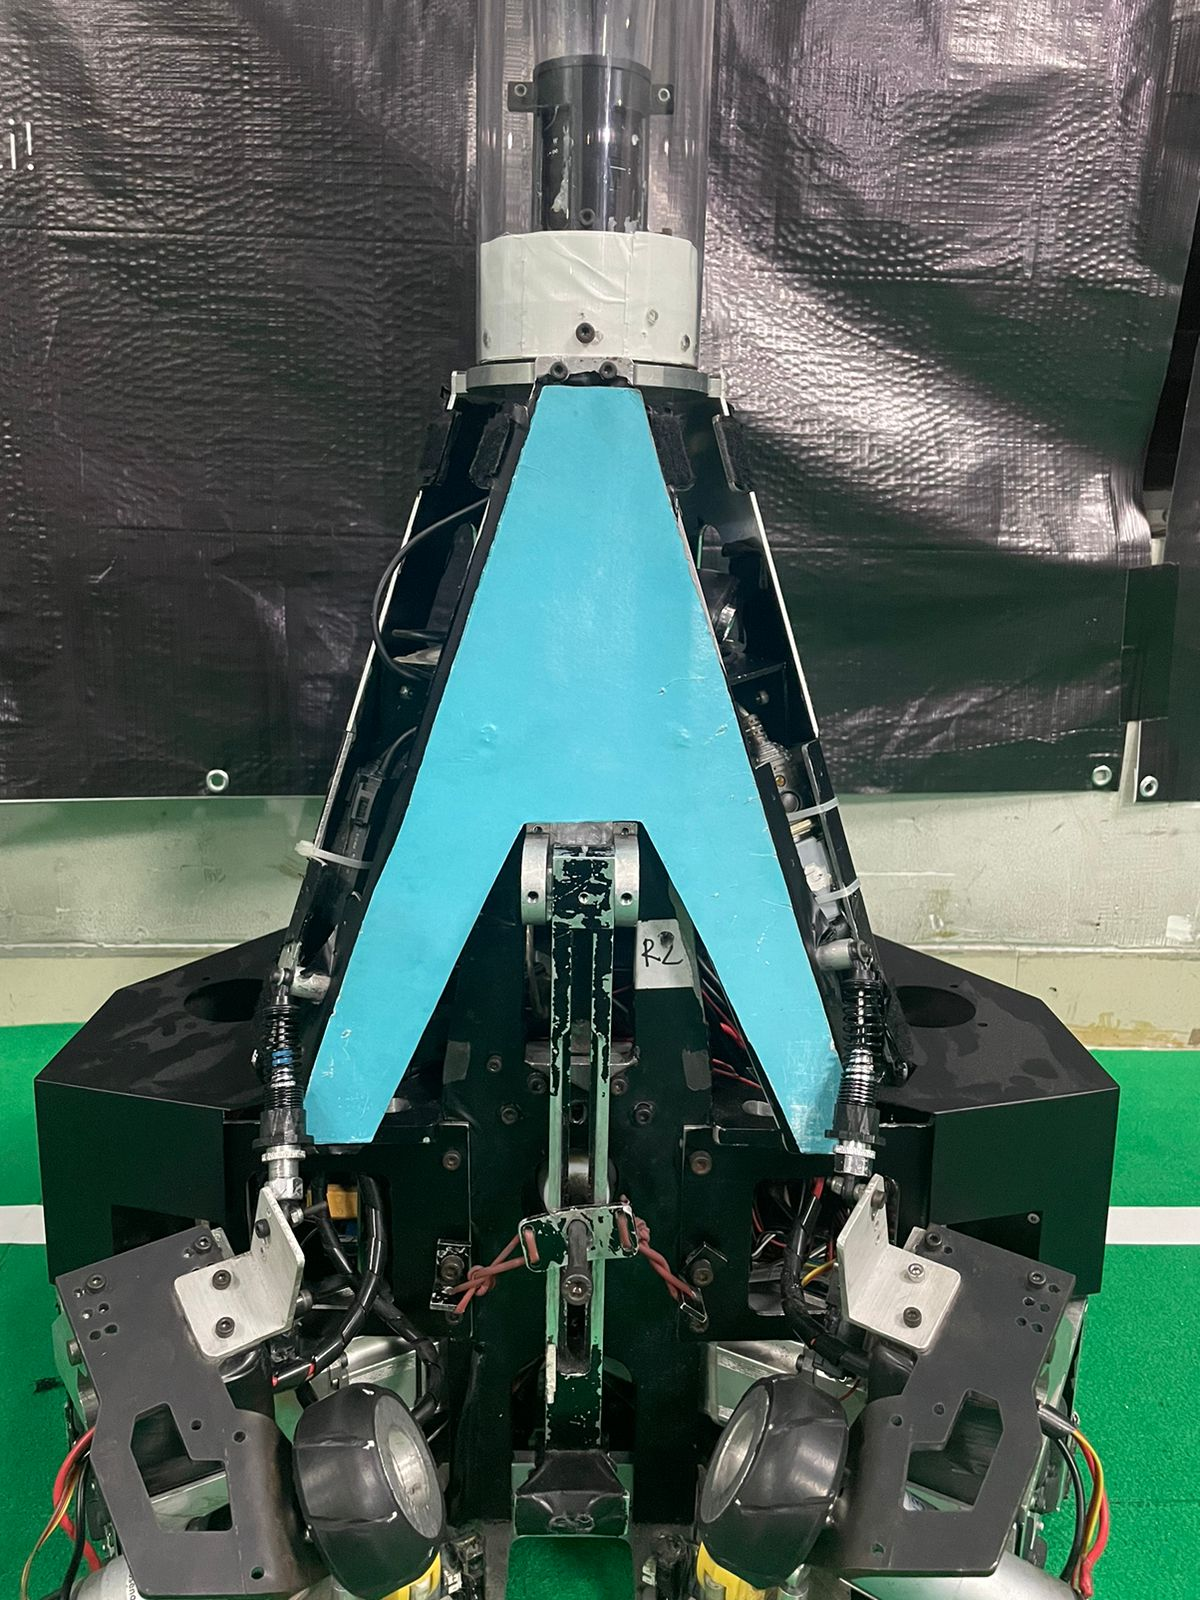
\includegraphics[width=6cm]{gambar/iris1.jpeg}
  
    % Ubah dengan keterangan gambar yang diinginkan
    \caption{IRIS Robot.}
    \label{fig:mobile_robot}
\end{figure}
Mobile Robot is a robot designed to move or move easily. The performance of the Mobile Robot is largely focused on tracking systems, localization, and algorithms. All of these are based on good sensing capabilities \citet{ref_mobile_robot}.

Sensor that commonly used in Mobile Robot is camera. The camera can be a regular camera or an Omnivision Camera. The use of Omnivision Camera can make the robot see in all directions, but the pre-processing of the data is more difficult than a regular camera.

\subsubsection{\emph{OpenCV}}
\label{sec:opencv}
% \begin{figure}[ht]
%     \centering
  
%     % Ubah dengan nama file gambar dan ukuran yang akan digunakan
%     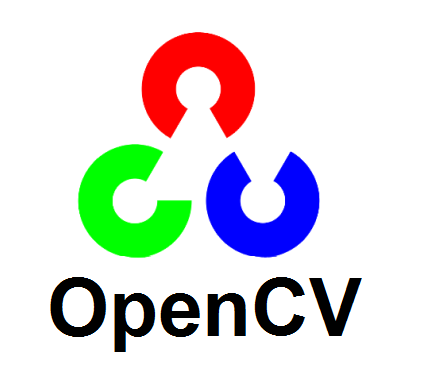
\includegraphics[width=8cm]{gambar/opencv.png}
  
%     % Ubah dengan keterangan gambar yang diinginkan
%     \caption{Logo OpenCV.}
%     \label{fig:opencv}
% \end{figure}

OpenCV is an open-source library developed by Intel with the C/C++ programming language. OpenCV provides many algorithms related to Computer Vision \citet{ref_opencv}. OpenCV is widely used for object detection based on color, shape, size, and other needs of the program.

\subsubsection{Robot Operating System}
\label{sec:ros}
% \begin{figure}[ht]
%     \centering
  
%     % Ubah dengan nama file gambar dan ukuran yang akan digunakan
%     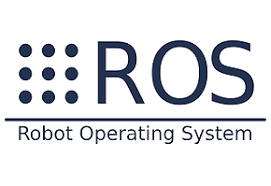
\includegraphics[width=8cm]{gambar/ros.png}
  
%     % Ubah dengan keterangan gambar yang diinginkan
%     \caption{Logo ROS.}
%     \label{fig:ros}
% \end{figure}

ROS or Robot Operating System is a platform that stands on Linux and is useful for synchronizing parts of the robot \citet{ref_ros}. ROS is widely used as the core of processing data from a robot starting from processing sensor data to becoming actuator data. ROS provides modular programming concepts with a publish/subscribe method for its IPC (Inter Process Communication). In addition to facilitating data transfer between processes, ROS also provides a timer with a default scheduler that follows the Default Linux Scheduler, namely the Priority-based scheduler. This allows users to set the priority of each part of their robot.

\subsubsection{Websocket}
\label{sec:websocket}
Websocket is a type of communication protocol based on the TCP protocol (Transmission Control Protocol). The websocket protocol makes both the sender and receiver always open their sockets so that they can communicate with each other. Compared to HTTP (Hypertext Transfer Transfer Protocol), the Websocket protocol has better latency \citet{ref_websocket}. Websocket applications are widely used for chat applications, online games, applications that require real-time data, and many others.
